\chapter{Convolutional Neural Networks}

Images have the key properties of translation invariance (the meaning of an image should not change if translated in the image plane) and translation equivariance (the image representation should change in a predictable way when the image is translated). Convolutional Neural Networks are a specialized Neural Network architecture that is used to work with grid data (images) as the input. Therefore these architectures, should be able to respect both translation invariance and translation equivariance.

\section{Convolutional Neural Network Architecture}

The Convolutional Neural Network architecture is composed of the following elements:

\begin{itemize}
    \item Input layer. As with Feedforward Neural Networks, this layer takes the input data. Instead of having a neuron for every attribute, in a Convolutional Neural Network each neuron represents the value of a pixel of the image making the size of the input layer (dimensionality) very big.
    \item Convolutional Layer. These ones apply a set of learnable filters (kernels) to the data. Each filter is convoluted with the data which consists of performing an element-wise multiplication of the filter values with the corresponding input data values and then summing up the results and applying a non-linear activation function. This results in a set of feature maps for each filter that captures different patterns or features of the input data. Convolutional layers help to extract spatial hierarchies of features from the input data.

    \begin{figure}[h]
        \centering
        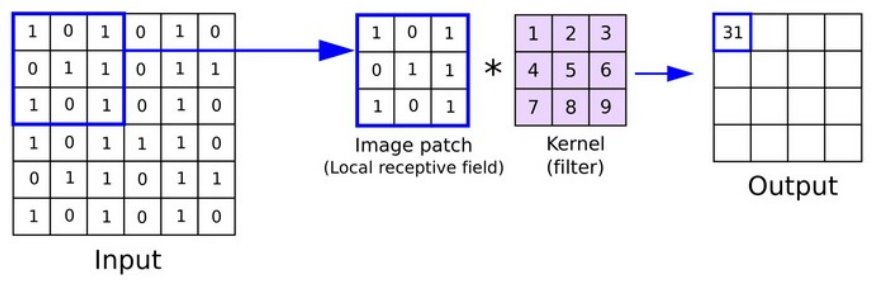
\includegraphics[width=12cm]{Images/convolutional-layer.jpg}
        \caption{Convolutional layer are used to create a feature map}
    \end{figure}

    We can perform the convolutional operation with a certain stride. This is the step size at which the filter moves across the input data. Having a stride different than 1 makes the size of our image to reduce by this factor. Instead, if it is only 1 the dimensionality of the next layer will be N - filter size + 1.

\newpage
    \item Pooling Layer. After the convolutional layer a pooling layer is usually applied to the set of feature maps that we get as the output of the convolutional layer. This pooling layer consists in performing some pooling operation (the most common one of which is max-pooling) to the output of the convolutional layer in order to reduce its size (down-sampling). Pooling helps make the representation become approximately invariant to small translations of the input.

    \begin{figure}[h]
        \centering
        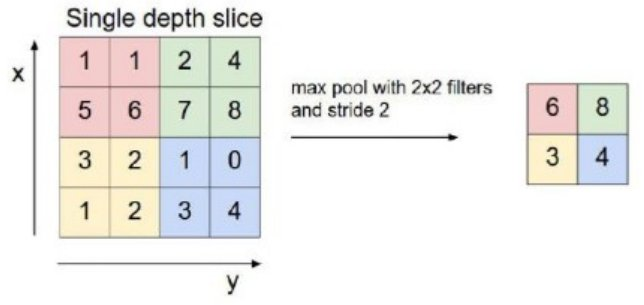
\includegraphics[width=8cm]{Images/max-pooling.jpg}
        \caption{Max pooling}
    \end{figure}
    In pooling we can also specify a certain stride which determines the step size at which the pooling kernel moves across the input data. A stride of k will reduce the image size by a factor of k.

    \item Fully Connected Layer. Usually at the end of the Convolutional Neural Network after a set of convolutional and pooling layers a fully connected layer is implemented. As in FNN this consists in connecting all the input neurons with all the output layer units. An activation function is applied in order to give the output of the Convolutional Neural Network.
    \begin{figure}[h]
        \centering
        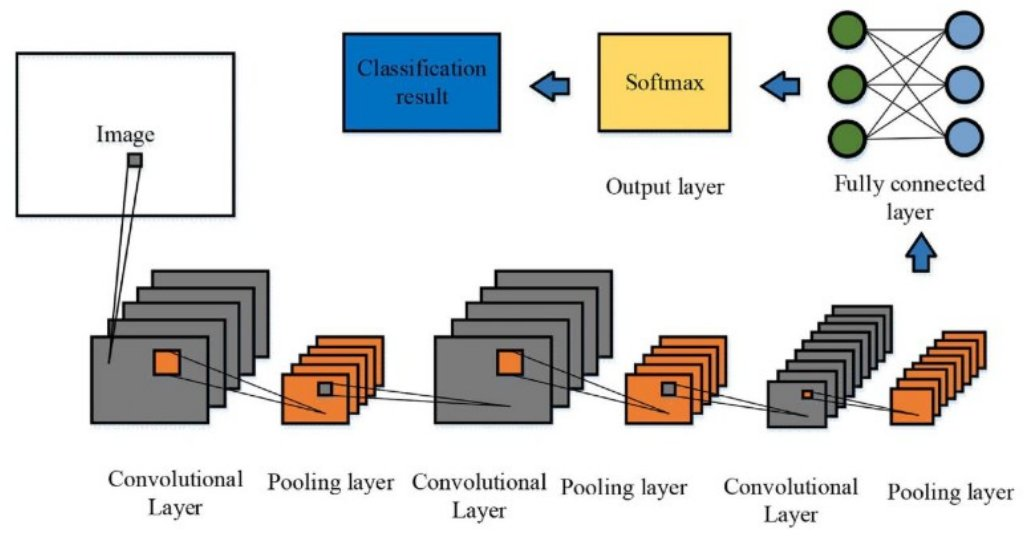
\includegraphics[width=10cm]{Images/cnn.jpg}
        \caption{Convolutional Neural Network Architecture}
    \end{figure}

    Notice that this fully connected layer takes the flattened set of feature maps from the preceding convolutional and pooling layers as input. In this way we will be able to make predictions or classifications based on the features learned by the preceding layers.

    After having the output we will be able to compare the output of our Convolutional Neural Network with the labels and build our loss function. With the loss function then we will perform backpropagation in order to update the parameters. This process is repeated for a number of N epochs.

\end{itemize}

\newpage
\section{Convolution Main Properties}

Convolution leverages two important features: local connectivity and parameter sharing. Let’s review them.

\begin{itemize}
    \item Local Connectivity. Due to the filter kernel being much smaller than the input data we will have only local connectivity. Therefore a point in the output feature map of the convolutional layer is only influenced by a small subset of nearby points in the input data. In a deep Convolutional Neural Network, units in the deeper layers may indirectly interact with a larger portion of the input. This allows the network to efficiently describe more complex interactions of the data by detecting combinations of the features that the previous layer have build.

    \begin{figure}[h]
        \centering
        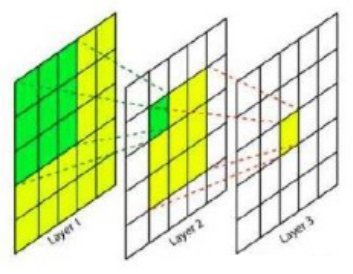
\includegraphics[width=4cm]{Images/local-connectivity.jpg}
        \caption{Local Connectivity}
    \end{figure}

    \item Parameter Sharing. Contrary to traditional Neural Networks in a Convolutional Neural Network each member of the kernel (filter) is used for every position of the input. So, instead of learning a separate set of parameters for every location we learn only one set per filter for every convolutional layer. This makes convolution more efficient than dense matrix multiplication and it also makes our model equivariance to translation (variations in the image data will also produce the same kind of variation in the output data).
    \begin{figure}[h]
        \centering
        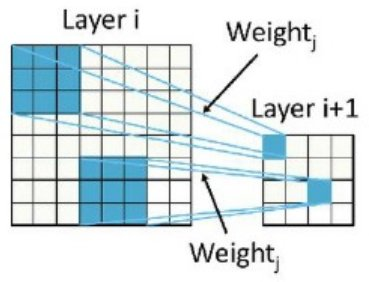
\includegraphics[width=4cm]{Images/parameter-sharing.jpg}
        \caption{Parameter Sharing}
    \end{figure}

\end{itemize}

\newpage
\section{Variants of the Basic Convolution Function}
\subsection{Padding}

One essential feature of any convolutional network implementation is the ability to implicitly zero-pad the input V in order to make it wider. Zero padding the input allows us to control the kernel width and the size of the output independently. This is basically done to not lose information with the pixels around the edges of the image. We have two types of padding: Valid padding and Same padding.

\begin{figure}[h]
    \centering
    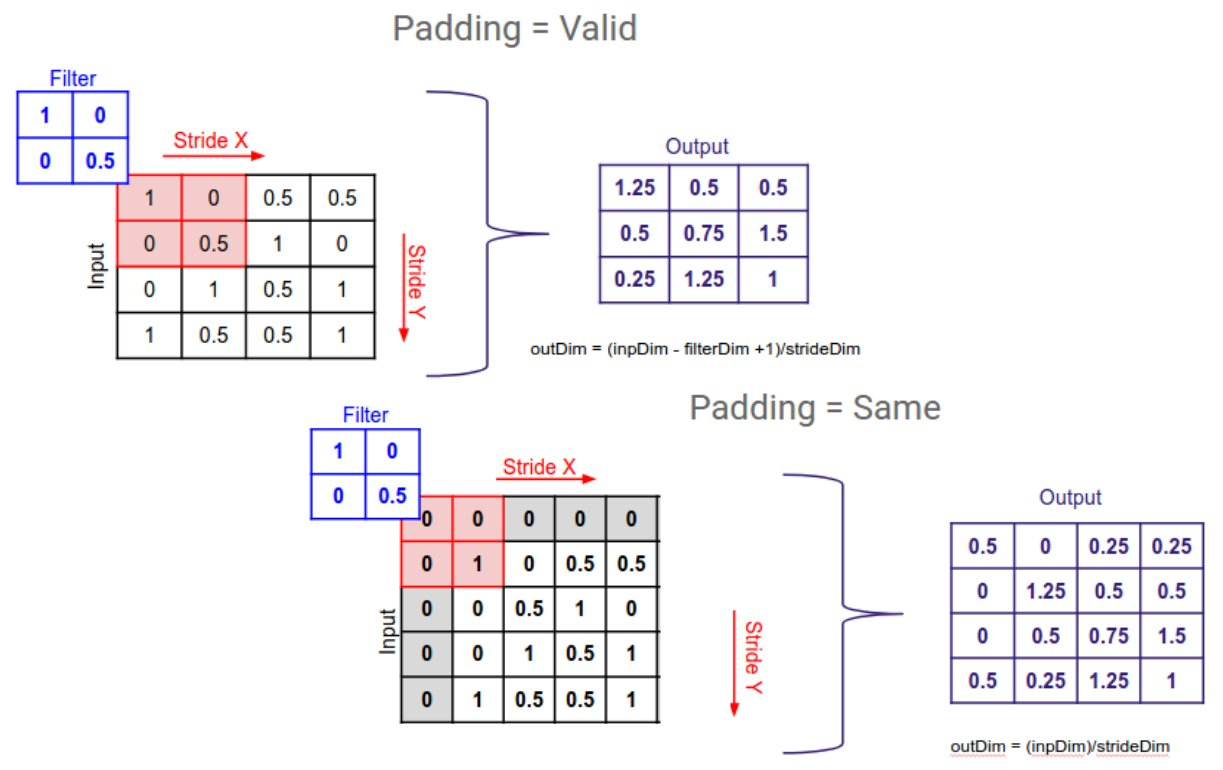
\includegraphics[width=10.5cm]{Images/padding.jpg}
    \caption{Padding}
\end{figure}

\begin{itemize}
    \item Valid padding consists of not applying any padding whatsoever. In this case, the size of the input shrinks at each layer. If the input image has width $m$ and the kernel has width $k$, the output will be of width $m - k + 1$.
    \item Same padding on the other hand consists of adding just enough zeros to keep the size of the output equal to the size of the input. However, the input pixels near the border influence fewer output pixels than the input pixels near the center so it can still make the border pixels somewhat underrepresented in the model.
\end{itemize}

\newpage
\subsection{Multichannel Inputs}

In the context of images, a single-channel image represents gray-scale intensity values, however, images can also have multiple channels, representing the three primary colors known as RGB channels. In this case, the convolutional filters are 3D, adding to the width and height dimensions also the number of channels. During the convolution operation, the filters slide across the input volume, computing element-wise multiplications with the corresponding input values from all channels and summing them to produce the output.

\begin{figure}[h]
    \centering
    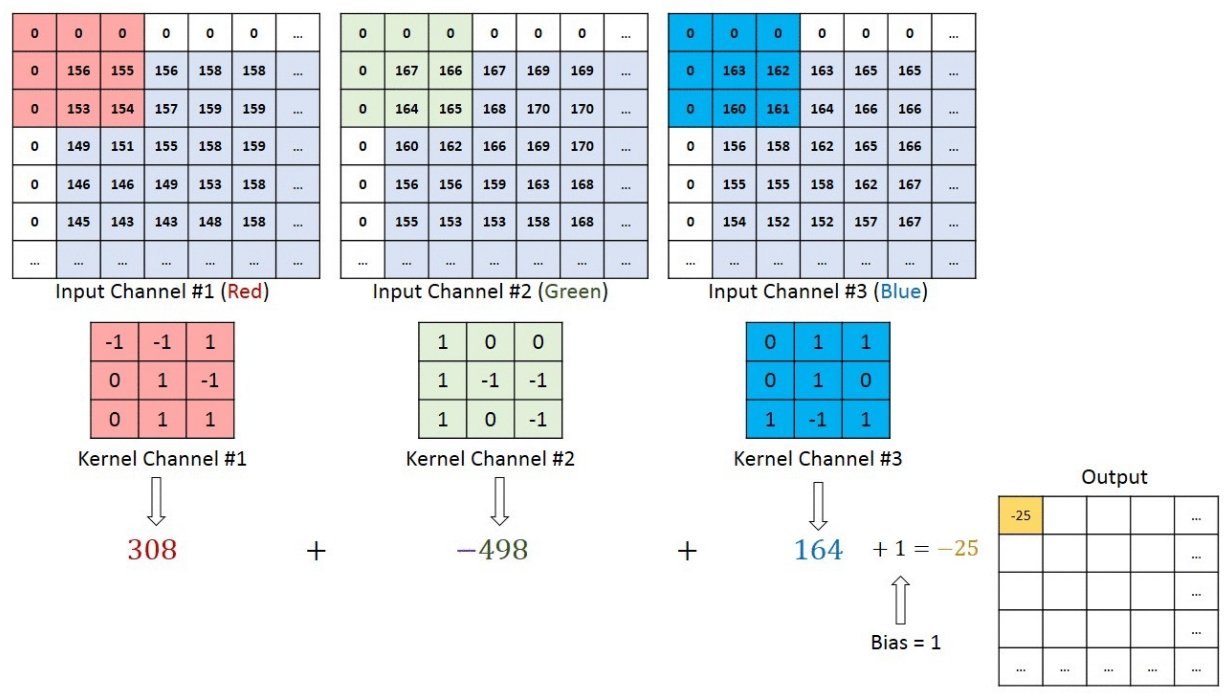
\includegraphics[width=15cm]{Images/rbg-filters.jpg}
    \caption{Multichannel inputs}
\end{figure}

